\documentclass[11pt,letterpaper]{article}
\usepackage{../assets/scientific_report}
\usepackage{amsmath}
\usepackage{float}
\usepackage{listings}
\usepackage{xcolor}
\usepackage{graphicx}
\usepackage{geometry}
\geometry{headheight=23pt, top=2cm, bottom=2cm, left=2.5cm, right=2.5cm}
\setlength{\parskip}{0.5em}
\setlength{\parindent}{0pt}
\lstset{
  language=C,
  basicstyle=\ttfamily\small,
  keywordstyle=\color{blue}\bfseries,
  commentstyle=\color{green!60!black}\itshape,
  stringstyle=\color{red!80!black},
  numbers=left,
  numberstyle=\tiny\color{gray},
  numbersep=8pt,
  frame=single,
  breaklines=true,
  captionpos=b,
  tabsize=4,
  showstringspaces=false,
  inputencoding=utf8,
  extendedchars=true,
  literate={ã}{{\~a}}1 {õ}{{\~o}}1 {á}{{\'a}}1 {à}{{\`a}}1 {â}{{\^a}}1 {é}{{\'e}}1 {ê}{{\^e}}1 {í}{{\'i}}1 {ó}{{\'o}}1 {ô}{{\^o}}1 {ú}{{\'u}}1 {ç}{{\c{c}}}1 {Ã}{{\~A}}1 {Õ}{{\~O}}1 {Á}{{\'A}}1 {É}{{\'E}}1 {Í}{{\'I}}1 {Ó}{{\'O}}1 {Ô}{{\^O}}1 {Ú}{{\'U}}1 {Ç}{{\c{C}}}1 {—}{{---}}1
}
\begin{document}
\pagestyle{plain}
\begin{center}
{\LARGE\bfseries Difusão viscosa 2D: particionamento e balanceamento de carga}\\[0.4em]
{\normalsize Eugenio Vitor Lopes dos Santos}\\[0.3em]
{\small DCA3703, Programação Paralela, Universidade Federal do Rio Grande do Norte}\\[0.3em]
\end{center}
\section{Enunciado}
\begin{quote}
``Escreva um código que simule o movimento de um fluido ao longo do tempo usando a equação de Navier-Stokes, considerando apenas os efeitos da viscosidade. Desconsidere a pressão e quaisquer forças externas. Utilize diferenças finitas para discretizar o espaço e simule a evolução da velocidade do fluido no tempo. Inicialize o fluido parado ou com velocidade constante e verifique se o campo permanece estável. Em seguida, crie uma pequena perturbação e observe se ela se difunde suavemente. Após validar o código, paralelize-o com OpenMP e explore o impacto das cláusulas \texttt{schedule} e \texttt{collapse} no desempenho da execução paralela.''
\end{quote}

\section{Fundamentação teórica}

\subsection{Particionamento de dados e divisão de trabalho}
Particionamos o domínio em partes e atribuímos cada parte às threads. No stencil desta tarefa, todas as células internas executam a mesma operação sobre os vizinhos. A divisão natural é espacial, por linhas ou por células. O equilíbrio depende do tempo de cada parte, não apenas do número de iterações. Se o custo for uniforme, uma divisão uniforme tende a funcionar bem. Custos diferentes fazem algumas threads esperar pelas outras.

Em OpenMP, \texttt{parallel} cria a equipe de threads. \texttt{for} distribui as iterações de um laço dentro dessa equipe, sem criar outra equipe. Um laço C comum dentro da região paralela é executado por todas as threads que o encontram. Se envolvêssemos o stencil apenas com \texttt{parallel}, cada thread repetiria as atualizações e o programa teria corridas.

\subsection{Divisão de blocos com \texttt{sections}}
A diretiva \texttt{\#pragma omp sections} distribui blocos estruturados, marcados por \texttt{section}, entre as threads da equipe. Cada bloco executa uma vez, mas uma mesma thread pode receber mais de um bloco. A implementação decide a atribuição. O programador não deve presumir a ordem textual nem um ID fixo de thread. A construção inclui uma barreira no final, salvo quando usamos \texttt{nowait}.

\begin{lstlisting}[language=C,caption={Exemplo conceitual de sections, não utilizado nas sete versões}]
#pragma omp parallel sections
{
    #pragma omp section
    { /* calcular um diagnostico independente */ }
    #pragma omp section
    { /* calcular outro diagnostico independente */ }
}
\end{lstlisting}

\texttt{sections} divide blocos de operações. \texttt{for} divide as iterações de um laço. Duas seções permitem no máximo duas threads executando esses blocos ao mesmo tempo, mesmo que a equipe seja maior. Uma seção longa não é subdividida para ocupar threads ociosas. \texttt{schedule} também não se aplica a \texttt{sections}.

Nesta grade, uma seção para cada região fixaria a decomposição no código. \texttt{for} ajusta a distribuição ao número de threads e ao tamanho da grade. Por isso, estudamos \texttt{sections}, mas não a usamos nas variantes. Para calcular diagnósticos independentes com essa construção, o campo teria de estar pronto e cada bloco teria de escrever em um destino próprio.

\subsection{A cláusula \texttt{schedule}: static, dynamic e guided}
A cláusula \texttt{schedule(tipo, chunk)} agrupa as iterações lógicas em blocos contíguos e define como as threads recebem esses blocos. Ela não elimina dependências, não protege variáveis compartilhadas e não escolhe o núcleo onde cada thread roda. Afinidade e distribuição de iterações são decisões diferentes.

Com \texttt{schedule(static)} sem chunk explícito, o runtime divide as iterações em blocos aproximadamente iguais, com no máximo um bloco por thread. Os limites exatos podem variar entre implementações. A atribuição não depende da ordem em que as threads terminam. Essa política reduz o gerenciamento durante o laço e favorece acessos contíguos quando cada iteração representa uma linha da matriz.

Com \texttt{schedule(static, k)}, o runtime atribui os blocos de k iterações em ciclo, seguindo a ordem das threads. Para 16 iterações, quatro threads e k=2, a thread 0 recebe 0--1 e 8--9, enquanto a thread 1 recebe 2--3 e 10--11. As demais recebem os blocos restantes. Assim, static com chunk não garante um único intervalo contíguo por thread.

Com \texttt{schedule(dynamic, k)}, uma thread recebe um bloco e pede outro quando termina, enquanto houver blocos disponíveis. O último bloco pode ter menos de k iterações. Sem chunk explícito, k=1. A política ajuda quando o custo das iterações ou a velocidade das threads varia, mas cobra um despacho a cada bloco. Em uma carga uniforme, ela pode não ganhar de static.

Com \texttt{schedule(guided, k)}, as threads também pedem novos blocos ao terminar. Os blocos começam maiores e diminuem conforme o trabalho restante e o número de threads. k é o tamanho mínimo, salvo no último bloco. Não é um tamanho fixo. Sem k explícito, o mínimo é 1. A sequência exata depende da implementação. Guided reduz os despachos no começo e usa blocos menores no final, mas um bloco inicial caro ainda pode atrasar a equipe.

As versões definem as políticas diretamente nos pragmas. Alterar \texttt{OMP\_SCHEDULE} não muda esses laços, pois a variável só controla construções com \texttt{schedule(runtime)}. O número de threads é outro parâmetro. O programa o recebe de \texttt{OMP\_NUM\_THREADS} e registra o valor observado dentro da região paralela.

\subsection{Chunksize: compromisso entre overhead e equilíbrio}
O chunksize conta iterações lógicas. Não conta bytes, threads ou núcleos. Blocos pequenos oferecem mais pontos de redistribuição, mas aumentam o custo de gerenciamento e podem fragmentar a localidade. Blocos grandes amortizam esse custo, porém deixam menos unidades para distribuir e podem concentrar trabalho no final.

No stencil, todas as células fazem o mesmo número de operações. A flexibilidade extra de dynamic ou guided pode custar mais do que economiza. Só os tempos podem testar essa hipótese. Diferenças entre threads, interferência externa e acessos remotos à memória também alteram o equilíbrio.

\subsection{A cláusula \texttt{collapse}}
\texttt{collapse(2)} junta os dois laços espaciais em um único espaço lógico, que o \texttt{schedule} distribui. Sem collapse, \texttt{omp for} distribui apenas o laço externo i. Cada unidade é uma linha com N$-$2 células internas. Com collapse, cada unidade é um par (i,j), ou seja, uma célula.

Para a grade retangular desta tarefa, a linearização conceitual é
\[
q=(i-1)(N-2)+(j-1),\qquad 0\le q<(N-2)^2.
\]
O compilador não precisa calcular q explicitamente a cada atualização. Os laços têm limites definidos, são independentes, usam incremento unitário e seguem a forma canônica exigida. Collapse não cria threads, não altera a disposição da matriz e não remove dependências de dados.

Se N$-$2 for menor que o número de threads, a divisão por linhas deixa parte da equipe ociosa. Collapse pode expor mais trabalho. Quando já há muitas linhas, o ganho não é automático. É preciso considerar a nova granularidade, a geração de índices e a vetorização. O laço temporal fica fora da distribuição porque cada passo depende do campo anterior.

\subsection{Paralelismo vetorial com \texttt{simd}}
A diretiva \texttt{\#pragma omp simd} permite executar várias iterações com instruções SIMD. Uma instrução SIMD opera sobre vários elementos e usa a unidade vetorial de um núcleo. Ela não cria threads. \texttt{omp for} distribui trabalho entre threads. As duas formas podem ser combinadas.

Uma opção seria distribuir as linhas com \texttt{omp for} e aplicar \texttt{omp simd} ao laço interno j. Cada thread cuidaria de suas linhas e o núcleo processaria células contíguas em vetores. \texttt{omp for simd} combina as duas construções no mesmo espaço de iterações.

Os buffers separados tornam as atualizações espaciais independentes. Ler um vizinho do campo antigo não interfere na escrita de outra célula do campo novo. Essa propriedade favorece a vetorização. Se o programa atualizasse o mesmo buffer, a análise seria outra. Também não declaramos alinhamento de 64 bytes sem garanti-lo, pois \texttt{malloc} não oferece necessariamente esse alinhamento.

Nenhuma das sete versões contém uma diretiva simd explícita. O compilador ainda pode autovetorizar. A largura efetiva depende do alvo e das opções de compilação. Para medir esse efeito, criaríamos uma variante com simd, manteríamos as demais condições e consultaríamos o relatório de vetorização do compilador. No GCC, estas opções mostram otimizações realizadas e oportunidades perdidas:
\begin{lstlisting}[language=bash,caption={Opções de diagnóstico de vetorização para um experimento adicional}]
-fopt-info-vec-optimized -fopt-info-vec-missed
\end{lstlisting}
A ausência do pragma não prova que não houve SIMD. A presença do pragma também não prova que o código ficou mais rápido.

\subsection{Dependências, barreiras e custo paralelo}
A correção vem antes da escolha da política de distribuição. Em cada passo, todas as threads leem o buffer antigo e cada célula do buffer novo tem um único escritor. Entre passos há uma dependência RAW. O próximo passo precisa dos valores produzidos pelo atual. A barreira no final de \texttt{omp for} deixa o campo pronto antes da troca dos ponteiros.

A troca ocorre em \texttt{single}, executado por uma thread da equipe. Ela não precisa ser a thread principal. A barreira final faz todas as threads prosseguirem com os ponteiros já trocados. Sem a primeira barreira, a troca poderia ocorrer durante escritas pendentes. Sem a segunda, o próximo passo poderia começar antes de todas as threads verem os novos ponteiros. Um \texttt{critical} por célula não é necessário. Ele serializaria atualizações independentes.

O tempo paralelo reúne trabalho útil, distribuição dos blocos, espera por desbalanceamento, sincronização e acesso à memória. Para p threads, calculamos o speedup $S(p)=T_{seq}/T_p$ e a eficiência $E(p)=S(p)/p$. O caso ideal S(p)=p exige divisão perfeita e nenhum custo extra. Uma política pode equilibrar melhor o trabalho e ainda perder tempo no gerenciamento.

\subsection{Modelo numérico usado como carga de trabalho}
No modelo usado, ``apenas efeitos da viscosidade'' também significa omitir a advecção, a pressão e as forças externas. Resolvemos uma componente escalar da velocidade, não o sistema completo de Navier--Stokes incompressível. Para viscosidade constante, $\partial_t u=\nu\nabla^2u$.

O esquema FTCS em uma grade quadrada usa
\[
u^{n+1}_{i,j}=u^n_{i,j}+r(u^n_{i-1,j}+u^n_{i+1,j}+u^n_{i,j-1}+u^n_{i,j+1}-4u^n_{i,j}),\qquad r=\frac{\nu\Delta t}{h^2}.
\]
Usamos $\nu=0.1$, $\Delta t=0.2$ e $h=1$, logo $r=0.02$. Em duas dimensões, o esquema é estável quando $0\le r\le 1/4$. Para uma solução suave e uma integração estável, o erro global é $O(\Delta t+h^2)$.

Nos modos parado e constante, as bordas têm o mesmo valor do interior, zero e um, respectivamente. A perturbação é uma gaussiana de amplitude 0.1 e $\sigma=N/10$, com bordas nulas desde o início. Nesse modo, a soma pode diminuir porque a difusão leva valores até as bordas.
\section{Implementação}
\subsection{Organização das versões e sincronização}
Cada arquivo \texttt{v*.c} é um programa completo e independente. A duplicação facilita a comparação dos pragmas. O tamanho da grade e o número de passos são constantes nomeadas diretamente no código como \texttt{tamanho\_grid=512} e \texttt{num\_passos\_tempo=500}. Cada programa recebe apenas o modo inicial e um caminho opcional para exportar o campo. Ele valida esses argumentos e o retorno de \texttt{malloc}. Dois buffers separam a leitura do instante antigo da escrita do novo. As bordas são inicializadas nos dois buffers e permanecem fixas durante o laço temporal, sem escritas concorrentes nos cantos.

A versão sequencial compila sem OpenMP. As seis variantes paralelas comparam static, dynamic com chunk 16 e guided com mínimo 16. Cada política aparece com e sem collapse(2). Uma única região paralela contém todos os passos, então o programa não reentra em uma região paralela a cada passo. As barreiras continuam necessárias. O runtime também pode reutilizar as threads, em vez de criar threads do sistema operacional a cada região.

\texttt{default(none)} exige que o código declare os escopos das variáveis. Os ponteiros u e v são compartilhados, assim como \texttt{tamanho\_grid}, \texttt{num\_passos\_tempo}, r e o registro do número real de threads. Compartilhar um ponteiro não duplica o campo apontado. Os contadores declarados dentro da região e as variáveis locais c e tmp pertencem a cada thread. Tornar apenas os ponteiros private não criaria uma matriz privada inicializada.

Cada thread percorre o laço temporal com seu contador t local. Todas encontram os laços de distribuição na mesma ordem. O \texttt{omp for} atribui cada célula a uma única thread em cada passo. Dentro de \texttt{single}, tmp troca u e v sem copiar a matriz. A ausência de corridas vem da exclusividade das escritas espaciais e das duas barreiras. \texttt{schedule} só define a distribuição do trabalho.
\begin{table}[H]
\centering
\begin{tabular}{lll}
\hline
Versão & Política & Unidade distribuída \\
\hline
v0 & Sequencial & Sem distribuição \\
v1 & \texttt{static} & Linha \\
v2 & \texttt{static}, \texttt{collapse(2)} & Célula \\
v3 & \texttt{dynamic,16} & Bloco de 16 linhas \\
v4 & \texttt{dynamic,16}, \texttt{collapse(2)} & Bloco de 16 células \\
v5 & \texttt{guided,16}, \texttt{collapse(2)} & Bloco decrescente de células \\
v6 & \texttt{guided,16} & Bloco decrescente de linhas \\
\hline
\end{tabular}
\caption{Versões completas e independentes. Em guided, 16 é o tamanho mínimo, salvo o último bloco.}
\end{table}
\subsection{Compilação e execução}
\begin{lstlisting}[language=bash,caption={Compilação e execução a partir de tarefa11/}]
gcc -std=c11 -O2 -Wall -Wextra v0_seq.c -lm -o ns_v0
gcc -std=c11 -O2 -Wall -Wextra -fopenmp v1_static.c -lm -o ns_v1
./ns_v0 1
./ns_v0 2
OMP_NUM_THREADS=4 ./ns_v1 0 campo.txt
\end{lstlisting}
\section{Resultados}
\subsection{Validação numérica}
Compilamos as sete variantes com GCC e as opções \texttt{-std=c11}, \texttt{-O2}, \texttt{-Wall}, \texttt{-Wextra} e \texttt{-Werror}. Usamos \texttt{-fopenmp} apenas nas versões paralelas. Os testes aprovaram 30 comparações de campos completos de $512\times512$ entre as variantes. Foram verificados os três modos iniciais e, para a perturbação, execuções com 1, 2 e 4 threads. O campo parado permaneceu nulo, o campo constante permaneceu unitário e todas as versões paralelas produziram exatamente o mesmo campo da referência sequencial. Também verificamos a queda do pico gaussiano e a rejeição de entradas inválidas.

A Figura~\ref{fig:difusao} mostra a perturbação gaussiana antes e depois dos 500 passos. O pico diminui enquanto o raio quadrático médio aumenta, sem oscilações nem novos extremos, comportamento esperado para difusão viscosa estável.
\begin{figure}[H]
\centering
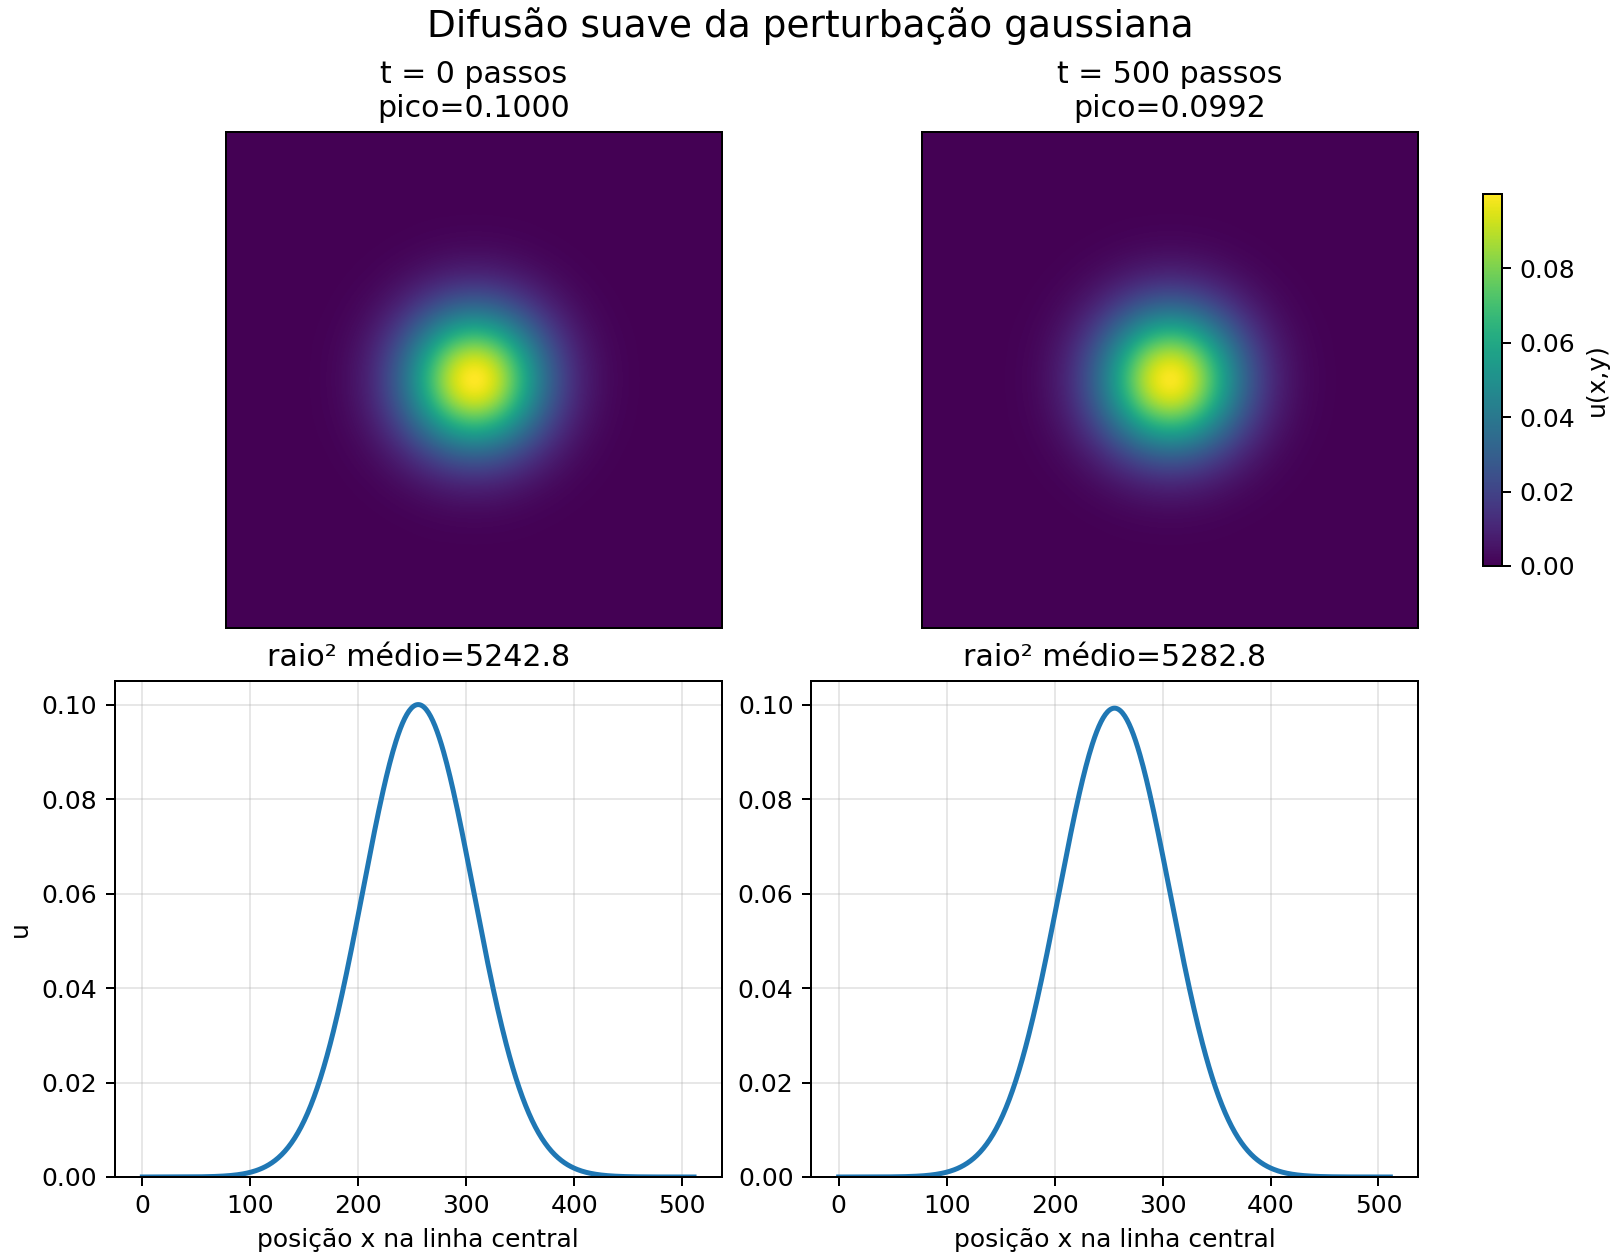
\includegraphics[width=0.95\textwidth]{visualizacao_difusao.png}
\caption{Difusão da perturbação gaussiana no início e após 500 passos.}
\label{fig:difusao}
\end{figure}
\subsection{Medição de desempenho}
O benchmark foi executado com GCC 13.3.0 no Intel Core i7-14700HX sob WSL2, usando uma grade $512\times512$, 500 passos e todas as quantidades de 1 a 28 threads disponíveis. Cada ponto de 1 a 25 threads usa a mediana de cinco repetições após aquecimento. Como a primeira varredura apresentou picos abruptos no final, os pontos de 26 a 28 threads foram repetidos dez vezes sob as mesmas condições e substituídos por essas medianas confirmadas. Foram usadas as opções \texttt{-std=c11}, \texttt{-O2}, \texttt{-Wall} e \texttt{-Wextra}, além de \texttt{-lm}; nas variantes paralelas, acrescentamos \texttt{-fopenmp}. Fixamos \texttt{OMP\_DYNAMIC=FALSE}, \texttt{OMP\_PROC\_BIND=close} e \texttt{OMP\_PLACES=cores}.

O cronômetro \texttt{CLOCK\_MONOTONIC} cobre a região paralela, o stencil, as barreiras e a troca de ponteiros. Ele não cobre alocação, inicialização ou exportação. A Tabela~\ref{tab:desempenho} apresenta medianas selecionadas; as Figuras~\ref{fig:tempo} e~\ref{fig:speedup} mostram toda a varredura e o speedup $S(p)=T_{seq}/T_p$. O conjunto consolidado está em \texttt{runs/resultado-confirmado/}; as duas execuções de origem permanecem preservadas para rastreabilidade.

\begin{table}[H]
\centering
\small
\resizebox{\textwidth}{!}{%
\begin{tabular}{lrrrrrr}
\hline
Versão & 1 thread & 2 threads & 4 threads & 8 threads & 14 threads & 28 threads \\
\hline
v1 static & 0,0970 & 0,0531 & 0,0289 & 0,0223 & 0,0207 & 0,0185 \\
v2 static + collapse & 0,1312 & 0,0722 & 0,0411 & 0,0326 & 0,0280 & 0,0488 \\
v3 dynamic & 0,1064 & 0,0621 & 0,0337 & 0,0220 & 0,0228 & 0,0276 \\
v4 dynamic + collapse & 0,2241 & 0,3662 & 0,3482 & 0,3342 & 0,3007 & 0,3225 \\
v5 guided + collapse & 0,1318 & 0,0706 & 0,0395 & 0,0277 & 0,0242 & 0,0329 \\
v6 guided & 0,1239 & 0,0588 & 0,0327 & 0,0240 & 0,0229 & 0,0269 \\
\hline
\end{tabular}%
}
\caption{Tempo mediano em segundos, selecionado da varredura completa de 1 a 28 threads. A referência sequencial teve mediana de 0,1049 s.}
\label{tab:desempenho}
\end{table}

\begin{figure}[H]
\centering

\includegraphics[width=0.98\textwidth]{tempo_execucao_log_plot.png}
\caption{Tempo mediano das políticas com e sem \texttt{collapse(2)}, de 1 a 28 threads, em escala logarítmica.}
\label{fig:tempo}
\end{figure}

\begin{figure}[H]
\centering

\includegraphics[width=0.98\textwidth]{speedup_plot.png}
\caption{Speedup relativo à referência sequencial. A reta tracejada representa o caso ideal.}
\label{fig:speedup}
\end{figure}

\subsection{Variação do chunksize}
Para separar o efeito de \texttt{collapse} do tamanho físico de cada bloco, realizamos um segundo experimento com oito threads. Sem collapse, os chunks foram 1, 4, 16 e 64 linhas. Com collapse, usamos 510, 2.040, 8.160 e 32.640 células, quantidades equivalentes a 1, 4, 16 e 64 linhas internas. Cada configuração teve cinco repetições; os dados estão em \texttt{runs/chunks-20260911-152008-206654/}.

\begin{figure}[H]
\centering
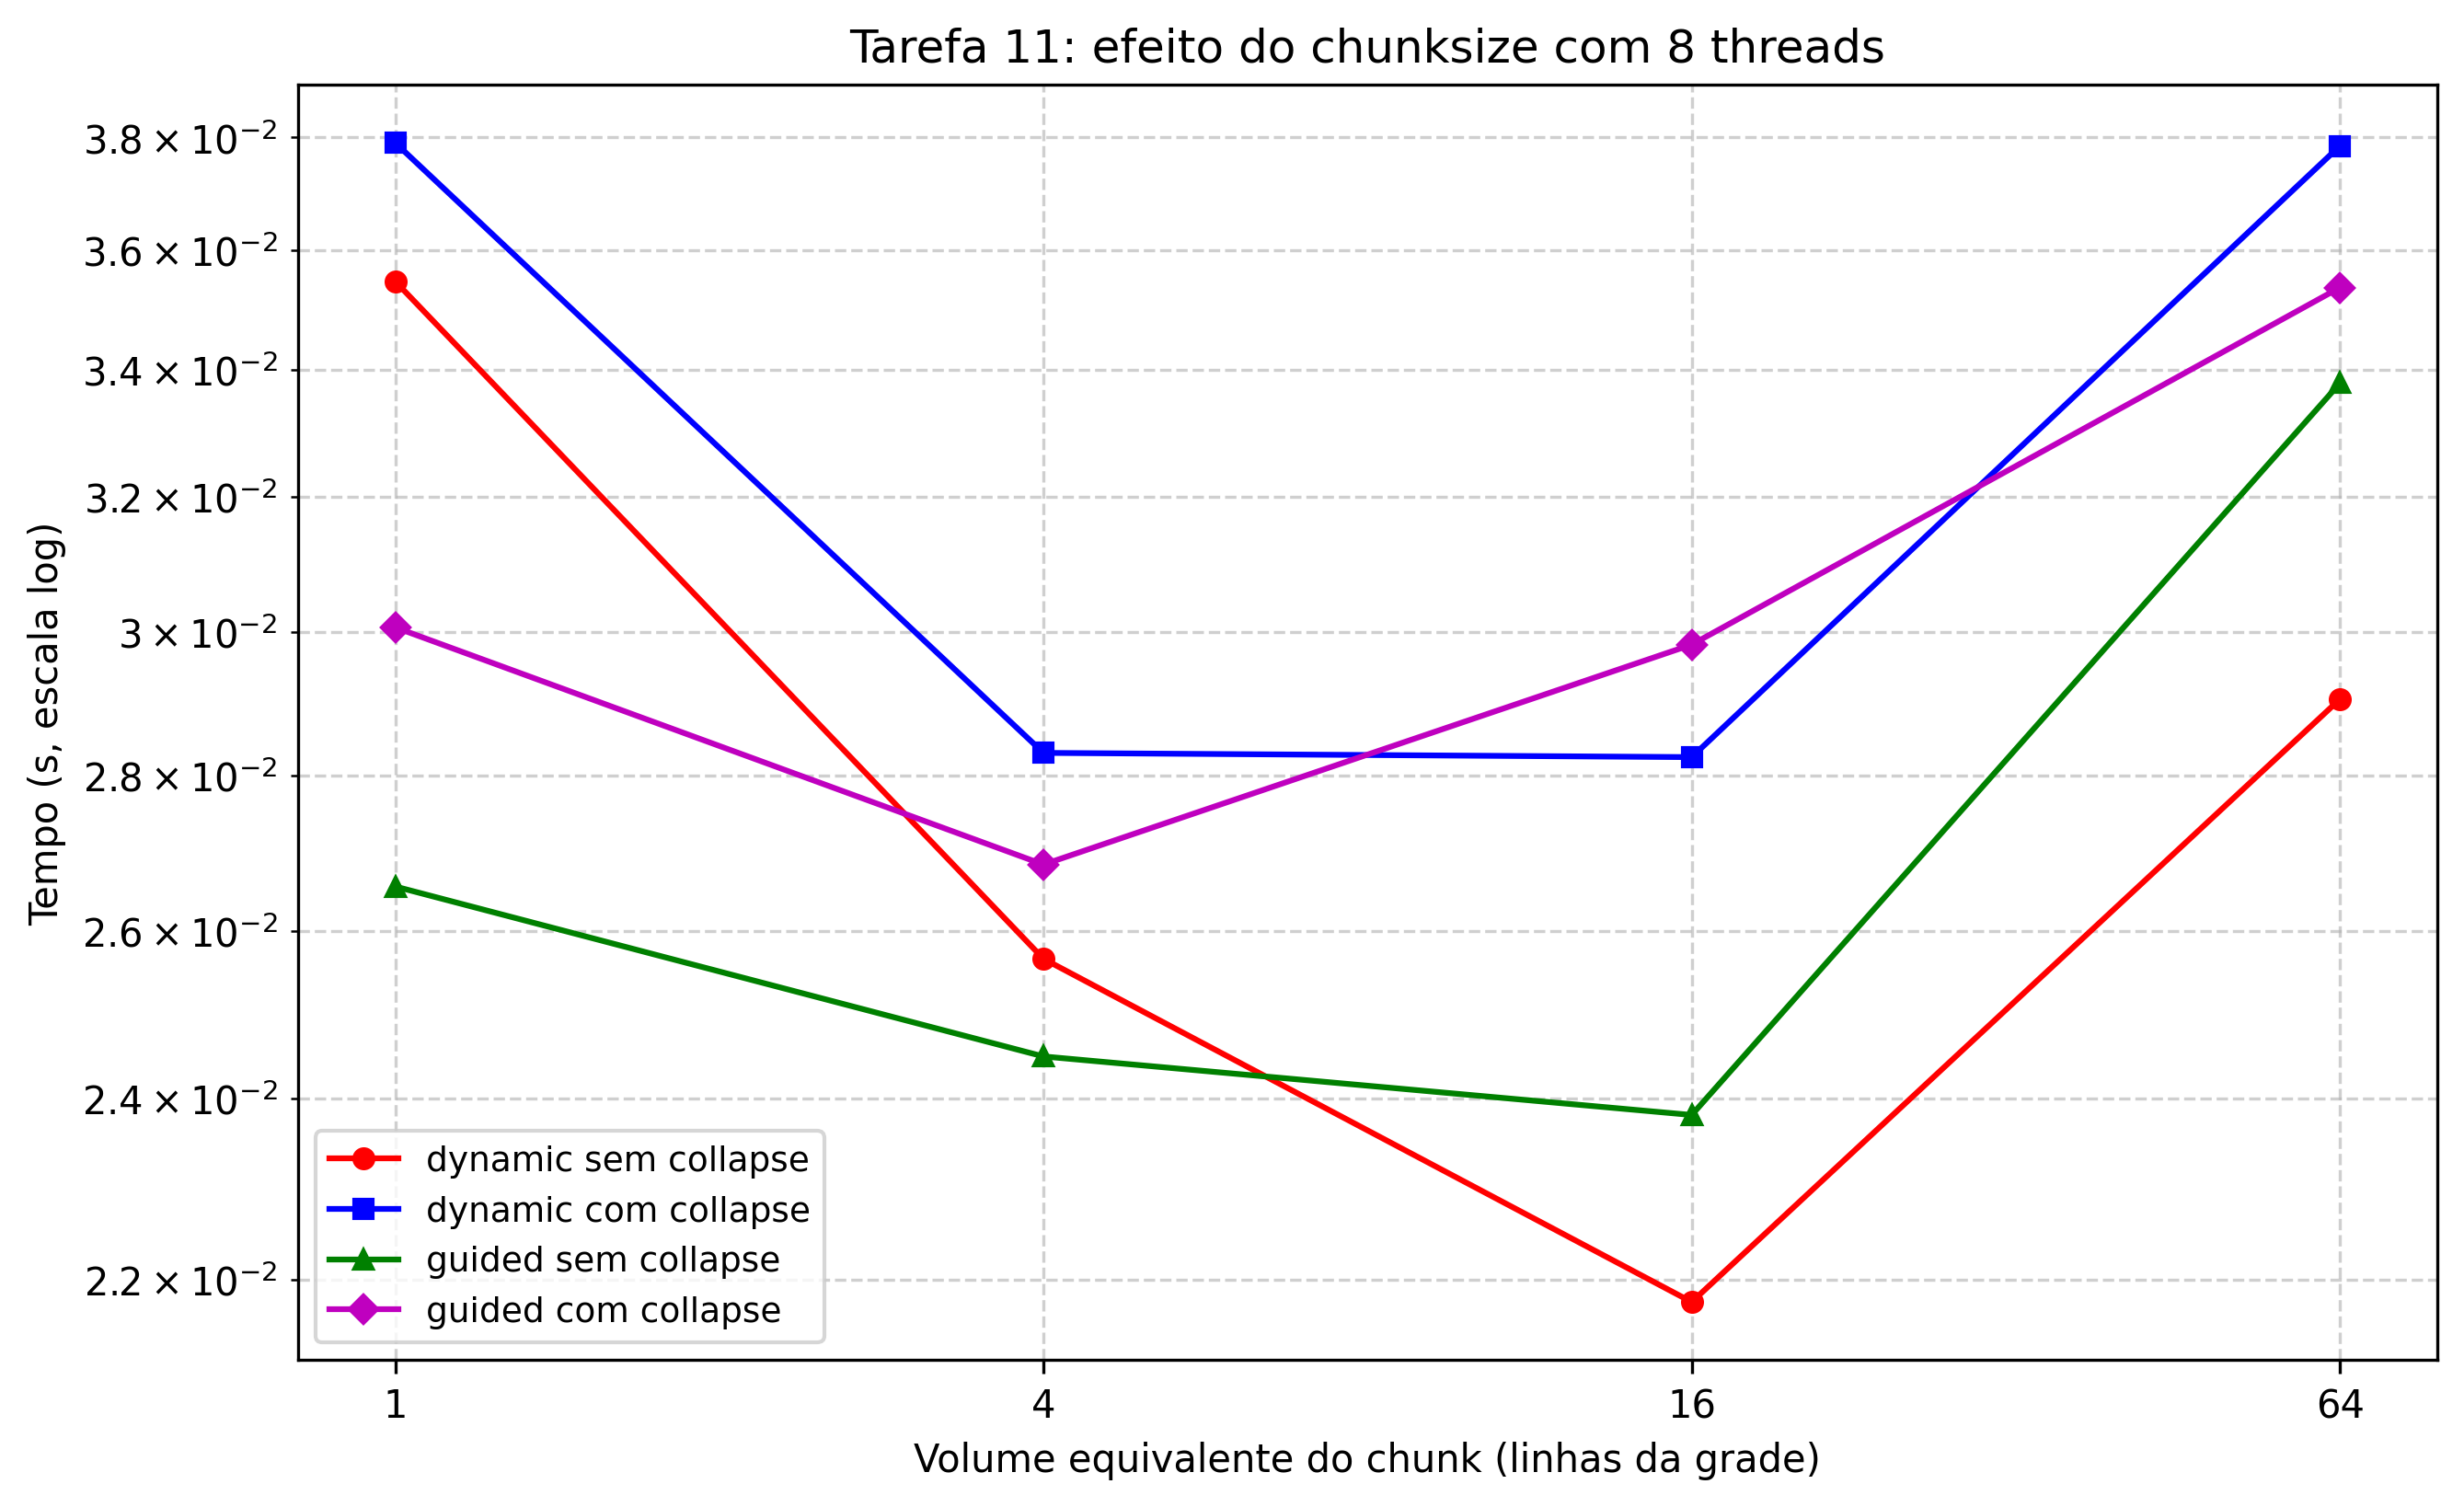
\includegraphics[width=0.92\textwidth]{chunksize_plot.png}
\caption{Efeito do chunksize com oito threads. O eixo horizontal representa o volume equivalente em linhas.}
\label{fig:chunks}
\end{figure}

No \texttt{dynamic}, o melhor resultado sem collapse ocorreu com 16 linhas por bloco (0,0218~s); com collapse, quatro e 16 linhas equivalentes ficaram próximos (0,0283~s). No \texttt{guided}, quatro linhas foi o melhor compromisso sem collapse (0,0245~s), enquanto uma linha equivalente foi melhor com collapse (0,0301~s). Chunks muito pequenos ampliaram o despacho; chunks de 64 linhas reduziram as oportunidades de balanceamento.
\section{Discussão}
\subsection{Granularidade e balanceamento}
Sem collapse, chunk 16 significa 16 linhas. Com collapse, significa 16 células. Para N=512, a grade tem 510 linhas internas e 260.100 células internas. Portanto, dynamic com chunk 16 distribui $\lceil510/16\rceil=32$ blocos por passo sem collapse e $\lceil260100/16\rceil=16.257$ com collapse. Esses números são blocos do laço, não threads ou tarefas novas.

No primeiro caso, cada bloco completo contém 8.160 atualizações. No segundo, contém apenas 16. Comparar dynamic,16 por linhas com dynamic,8160 por células aproximaria o volume de trabalho por bloco. Esse controle separa o custo de collapse do custo da granularidade. Em guided, o chunk é um mínimo, então a quantidade de blocos não segue essa divisão fixa.

Comparamos v1 com v2, v3 com v4 e v6 com v5 para estudar collapse dentro de cada política. A comparação entre v1, v3 e v6 mantém a distribuição por linhas. A comparação entre v2, v4 e v5 mantém a distribuição por células. Para comparar tempos, mantemos N, o número de passos, o modo inicial, o compilador e a equipe. Resultados numéricos iguais confirmam os casos testados, mas não mostram que o trabalho foi distribuído de modo igual.

\subsection{Localidade e limites de escalabilidade}
Com quatro threads, \texttt{static} sem collapse obteve o menor tempo: 0,0289~s e speedup 3,63. Na varredura completa, o menor tempo global foi 0,0183~s com \texttt{static} sem collapse e 16 threads, correspondente a speedup 5,72. \texttt{dynamic} e \texttt{guided} sem collapse atingiram seus menores tempos com 12 threads, respectivamente 0,0217~s e 0,0219~s. A carga uniforme favorece a política estática, que distribui as linhas com pouco gerenciamento. C armazena a matriz em ordem row-major; variar j acessa posições contíguas e reutiliza vizinhos no cache, e blocos de linhas preservam essa localidade.

O impacto de \texttt{collapse(2)} foi predominantemente negativo nesta configuração. Até mesmo \texttt{static} com collapse passou para 0,0411~s com quatro threads. O pior caso foi \texttt{dynamic,16} com collapse: 0,3482~s e speedup 0,30. Sem collapse, cada chunk reúne 16 linhas; com collapse, reúne somente 16 células. Para $N=512$, isso aumenta de 32 para aproximadamente 16.257 blocos por passo. O custo de milhões de despachos ao longo dos 500 passos supera o trabalho útil. \texttt{guided} reduz esse problema usando blocos inicialmente maiores, mas sua versão com collapse ainda foi mais lenta que a divisão por linhas.

Em uma linha de cache de 64 bytes cabem oito doubles. Threads que escrevem células distintas na mesma linha podem provocar falso compartilhamento, mesmo sem disputar a mesma célula. O efeito depende dos limites dos blocos e do alinhamento. Chunk 16 não o elimina em todos os limites de linha da matriz.

Cache, banda de memória, barreiras e afinidade podem limitar a escala. Os dois buffers da grade $512\times512$ ocupam 4 MiB e podem caber em cache. Por isso, speedup baixo não prova saturação da RAM. Após aproximadamente 16 threads, a versão static sem collapse entrou em um platô: 0,0183~s com 16 threads e 0,0185~s com 28. As demais políticas deixaram de melhorar antes disso. Os picos inicialmente observados em 26--28 threads não se repetiram de forma sistemática no ensaio de confirmação, mostrando a importância de repetir medições em ambiente virtualizado. Ainda assim, barreiras, gerenciamento OpenMP, SMT e os núcleos híbridos do processador limitam o ganho nessa carga curta.

\subsection{Papel de sections e simd nesta aplicação}
Não usamos sections porque o trabalho principal é um conjunto grande de atualizações iguais, não poucos blocos de funções diferentes. SIMD atua dentro do núcleo e pode complementar a divisão entre threads. Como não incluímos uma variante simd nem medimos a vetorização, os resultados não permitem atribuir ganhos a essa diretiva. Essa distinção separa os conceitos discutidos das técnicas avaliadas.

\section{Conclusão}
Os testes preservaram os campos zero e unitário e verificaram a difusão da perturbação sem criar novos extremos. As sete versões produziram campos idênticos nos casos testados. A região paralela persistente mantém as barreiras necessárias para atualizar o stencil e trocar os buffers.

A comparação entre políticas precisa considerar a unidade do chunk. Sem collapse, ela é uma linha; com collapse, é uma célula. Para esta carga uniforme e para a grade avaliada, \texttt{schedule(static)} sem \texttt{collapse} apresentou o melhor desempenho com quatro threads e também o menor tempo de toda a varredura, com 16 threads. O ganho saturou antes do máximo de 28 threads. A versão \texttt{dynamic,16} com collapse foi a menos adequada porque sua granularidade fina gerou overhead de distribuição muito superior ao trabalho de cada bloco.
\appendix
\newpage
\section{Código-fonte}
Apresentamos os arquivos completos para comparar diretamente as alterações de OpenMP.
\lstinputlisting[caption={v0\_seq.c: referência sequencial}]{v0_seq.c}
\newpage
\lstinputlisting[caption={v1\_static.c: static por linhas}]{v1_static.c}
\newpage
\lstinputlisting[caption={v2\_static\_collapse.c: static por células}]{v2_static_collapse.c}
\newpage
\lstinputlisting[caption={v3\_dynamic.c: dynamic por linhas}]{v3_dynamic.c}
\newpage
\lstinputlisting[caption={v4\_dynamic\_collapse.c: dynamic por células}]{v4_dynamic_collapse.c}
\newpage
\lstinputlisting[caption={v5\_guided\_collapse.c: guided por células}]{v5_guided_collapse.c}
\newpage
\lstinputlisting[caption={v6\_guided.c: guided por linhas}]{v6_guided.c}
\end{document}
